\documentclass[conference]{IEEEtran}
\IEEEoverridecommandlockouts

\usepackage{cite}
\usepackage{amsmath,amssymb,amsfonts}
\usepackage{algorithmic}
\usepackage{graphicx}
\usepackage{textcomp}
\usepackage{xcolor}
\def\BibTeX{{\rm B\kern-.05em{\sc i\kern-.025em b}\kern-.08em
    T\kern-.1667em\lower.7ex\hbox{E}\kern-.125emX}}
\begin{document}

\title{Inteligência Artificial no Processo de Seleção de Candidatos a Vagas de Emprego\\

}

\author{\IEEEauthorblockN{1\textsuperscript{st} Francisca Amanda Miranda de Paula}
\IEEEauthorblockA{\textit{Centro Universitário IESB} \\
\textit{Centro Universitário Instituto de Educação Superior de Brasília}\\
Brasília, Brasil \\
Matrícula - 1812082052}
\and
\IEEEauthorblockN{2\textsuperscript{nd} Matheus Henrique Santos Lucas}
\IEEEauthorblockA{\textit{Centro Universitário IESB} \\
\textit{Centro Universitário Instituto de Educação Superior de Brasília}\\
Brasília, Brasil \\
Matrícula - 1822082032}
}

\maketitle

\begin{resumo}
O presente projeto consiste em desenvolver um aplicativo na linguagem flutter, que inclui técnicas de inteligência artificial para selecionar automaticamente o candidato que se encaixa melhor com a oportunidade de emprego em questão. Para o desenvolvimento da aplicação, com o objetivo de ter um projeto mais limpo, organizado e fácil de receber manutenção, foram implementados alguns recursos, sendo eles: arquitetura limpa (Clean Architecture), padrão de projeto MVVM, spring boot e lombok na API em Java etc.
\end{resumo}

\begin{IEEEpalavrachave}
inteligência artificial, regressão linear, correlação linear.
\end{IEEEpalavrachave}

\begin{abstract}
The present project consists in developing an application in flutter language, that includes techniques of artificial intelligence to automatically select the candidate who best fits the job opportunity. For application development, with the goal to have a cleaner project, more organized and easier to receive maintenance, was implemented some resources, like: clean architecture (Clean Architecture), MVVM design pattern, spring boot and lombok frameworks in the API in the Java etc.
\end{abstract}

\begin{IEEEkeywords}
artificial intelligence, linear regression, linear correlation.
\end{IEEEkeywords}

\section{Introdução}
O uso da inteligência artificial dentro da área de recursos humanos traz muitos benefícios ao agilizar o processo de contratação, além de torná-los mais eficazes. Entre as diversas técnicas que podem ser aplicadas para implementar esta funcionalidade, existe a regressão linear que aprende a prever o melhor perfil treinando por meio de dados históricos que já vem com os resultados pré-definidos.

\section{Contextualização}

A candidatura às vagas de emprego geralmente é bastante concorrida pelo fato de ter muitos participantes para fazer a avaliação do perfil, tornando o processo de contratação lento na maioria das vezes. Sendo assim, é interessante agilizar o processo de seleção, visto que a demora pode prejudicar tanto a empresa quanto os interessados pela vaga. 

Portanto, muitas empresas quando estão contratando, ficam com certas demandas paradas somente esperando o novo funcionário assumir o cargo para então dar andamento e prosseguimento às tarefas, sendo que até o novo funcionário se adaptar às atividades leva algum tempo, o que pode levar ao atraso do cumprimento das demandas e regressão na produtividade da equipe como um todo. Quanto ao candidato, este permanece disponível para o mercado de trabalho por mais tempo do que deveria, perdendo até outras oportunidades de emprego. 

\section{Problema}
Definir a melhor estratégia e técnica da inteligência artificial para usá-la na pré-seleção de candidatos em uma vaga específica, além de decidir quais variáveis serão levadas em conta para análise e tomada de decisão, obtendo uma alta taxa de precisão. Neste contexto, como selecionar o melhor candidato com a menor taxa de erros possíveis, tendo em vista que a quantidade de parâmetros para medir as habilidades de um profissional, considerando também os requisitos, são praticamente infinitos?

\section{Objetivo Geral}
Desenvolver um aplicativo para dispositivos móveis com sistema operacional Android, que faz uso da inteligência artificial para realizar uma contratação inicial de candidatos em vagas de emprego. Assim, para resolver o problema exposto, será necessário utilizar um algoritmo que faz ligação de variáveis, para comparar os atributos do perfil candidato com os atributos de requisito das vagas. Portanto uma das técnicas estudada que atende melhor o objetivo final do projeto para se obter os resultados esperados, é o algoritmo de regressão linear da área de inteligência artificial.

\section{Objetivos Específicos}
\begin{itemize}
\item Desenvolver e consumir APIs; 
\item Usar padrões de projeto e boas práticas de programação, como os princípios S.O.L.I.D e Clean Architecture; 
\item Planejar e criar a interface do usuário;
\item Integrar o backend com a Interface do usuário (frontend); 
\item Desenvolver funcionalidades para cadastro e autenticação de usuários;
\item Conectar no banco de dados PostgreSQL;
\item Subir aplicação para o Heroku;
\item Aplicar a regressão linear para selecionar o candidato que é o mais apto para vaga de emprego;
\item Incluir chat bot e mapa no projeto.
\end{itemize}

\section{Referencial Teórico}
No trabalho proposto, será estudado o funcionamento do Algoritmo de Regressão Linear dentro do contexto de recrutamento para vagas de emprego. Assim, como a técnica de análise de perfil para seleção envolve a ligação entre variáveis que existem uma boa correlação entre si, a regressão linear consegue verificar o quanto uma variável está relacionada à outra, por exemplo, comparando as habilidades do candidato com os requisitos das vagas de emprego, fazendo um ajuste linear nos dados obtidos em um diagrama de dispersão, conforme mostra o gráfico abaixo:


\vspace{7mm}
\centerline{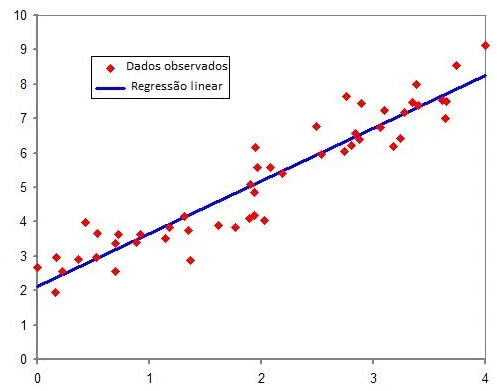
\includegraphics[width=80mm,height=600mm,keepaspectratio]{ExRegressaoLinear.png}}
\vspace{7mm}

\subsection{Regressão Linear}
A regressão linear é um algoritmo supervisionado que aprende a fazer previsões a partir de análises de dados históricos que já tenham resultados pré-definidos, passando a obter um modelo de referência do que pode estar certo ou errado. 

Para o procedimento da regressão linear aplicado na seleção de candidatos, é necessário utilizar um dataset que contenha dados históricos de um processo seletivo com a finalidade de treinar o algoritmo para que ele tenha a capacidade de prever os candidatos mais aptos para uma área específica. Para isso, será necessário definir quais serão as variáveis independentes, os atributos, que representam os requisitos e habilidades exigidas pela vaga em si.

Além disso, é necessário obter os valores da variável dependente, ou seja, o resultado da seleção individual de cada candidato. Por se tratar de resultados que possuem uma variável numérica, o método utilizado deverá ser o da regressão linear, pois para os casos em que o dado é categórico, utiliza-se a técnica de classificação linear.

Logo abaixo, tem-se um exemplo de um dataset voltado para vaga de Administrador de Banco de Dados (DBA):

\vspace{7mm}
\centerline{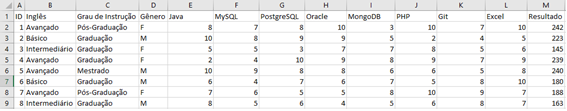
\includegraphics[width=90mm,height=600mm,keepaspectratio]{Tabela1.png}}
\vspace{7mm}

Para a regressão linear, todos os valores dos atributos deverão ser numéricos, pois é necessário realizar o cálculo da correlação linear de modo a medir o quanto aquela habilidade influência nos resultados. Este cálculo da correlação, serve para selecionar quais variáveis independentes devem ser levadas em consideração no teste e treinamento do algoritmo, de modo a minimizar as diferenças entre o resultado esperado e o obtido.

Após converter os dados categóricos em numéricos, tem-se a seguinte tabela:

\vspace{7mm}
\centerline{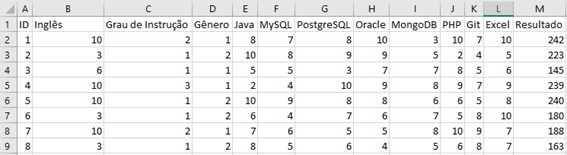
\includegraphics[width=90mm,height=600mm,keepaspectratio]{Tabela2.png}}
\vspace{7mm}

O próximo passo é calcular o valor da correlação cujo resultado varia entre -1 e 1. Assim, quanto mais próximo de 1, maior é a ligação da variável independente com a dependente (resultado), sendo congruente selecionar os requisitos que possuem estas características. Neste contexto, a correlação é classificada da seguinte forma:

\begin{itemize}
\item Correlação Positiva: valor igual ou próximo de 1.

\vspace{7mm}
\centerline{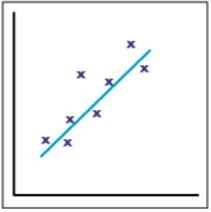
\includegraphics[width=60mm,height=40mm,keepaspectratio]{Diagrama1.png}}
\vspace{7mm}
\item Correlação Negativa: valor igual ou próximo de -1.

\vspace{7mm}
\centerline{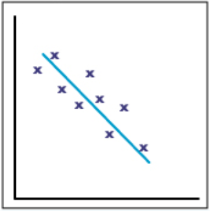
\includegraphics[width=60mm,height=40mm,keepaspectratio]{Diagrama2.png}}
\vspace{7mm}
\item Sem correlação: o resultado é igual a 0.

\vspace{7mm}
\centerline{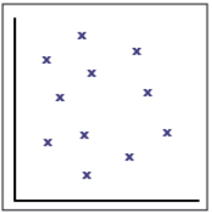
\includegraphics[width=60mm,height=40mm,keepaspectratio]{Diagrama3.png}}
\vspace{7mm}
\end{itemize}

Para os testes e treinamentos do algoritmo, serão levados em conta os atributos com correlação linear que são mais próximos de 1.

Utilizando a função “correl” fornecida pelo Excel para calcular a correlação linear entre cada variável independente com a dependente, foram encontrados os seguintes valores:

\vspace{7mm}
\centerline{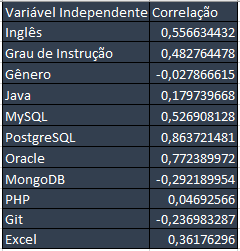
\includegraphics[width=60mm,height=40mm,keepaspectratio]{Tabela6.png}}
\vspace{7mm}

Abaixo, tem dois exemplos do diagrama de dispersão, sendo o primeiro uma correlação negativa e o segundo uma correlação positiva:

\vspace{7mm}
\centerline{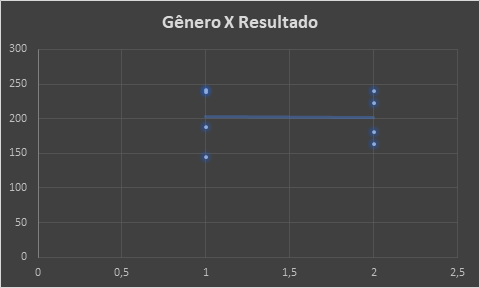
\includegraphics[width=60mm,height=40mm,keepaspectratio]{Grafico1.png}}
\vspace{7mm}

\vspace{7mm}
\centerline{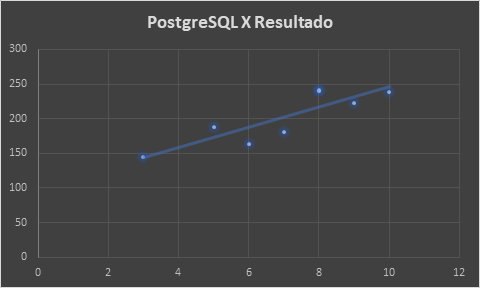
\includegraphics[width=60mm,height=40mm,keepaspectratio]{Grafico2.png}}
\vspace{7mm}

Após a obtenção dos resultados da correlação linear, foram excluídos os atributos que tinha valores próximos ou abaixo de 0, restando para análise as seguintes habilidades:

\vspace{7mm}
\centerline{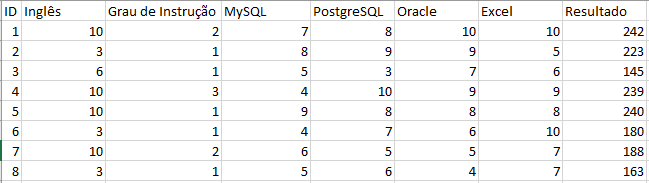
\includegraphics[width=60mm,height=40mm,keepaspectratio]{Tabela3.png}}
\vspace{7mm}

Para obter o valor de cada resultado, foram utilizados diferentes pesos em cada habilidade, sendo estes escolhidos pelos recrutadores, considerando o nível de relevância de cada requisito existente para a vaga. Para o caso de uma das habilidades do candidato não ser um dos requisitos da vaga, neste será atribuído peso igual a zero. Sendo assim, o procedimento para chegar até o resultado, consiste em multiplicar cada pontuação que está na tabela pelo peso da respectiva habilidade, somando tudo no final. A seguir, tem-se um exemplo para calcular o resultado para o candidato de ID igual a 1 utilizando como exemplo, o dataset abaixo:

\vspace{7mm}
\centerline{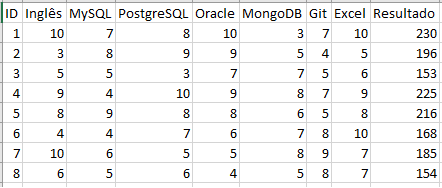
\includegraphics[width=60mm,height=40mm,keepaspectratio]{Tabela7.png}}
\vspace{7mm}

\vspace{7mm}
\centerline{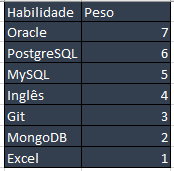
\includegraphics[width=60mm,height=40mm,keepaspectratio]{Tabela4.png}}
\vspace{7mm}

(4×10) + (5×7) + (6×8) + (7×10) + (2×3) + (3×7) + (1×10) = 230

O tipo de regressão linear abordada neste trabalho é a múltipla, pelo fato de possuir mais de uma variável independente. 

\section*{Trabalhos Correlatos}
Entre as inúmeras tecnologias existentes que automatizam processos, existem as que auxiliam no processo de contratação de candidatos às vagas de emprego. Como por exemplo, tem-se a ferramenta HireVue que é utilizada nas entrevistas online, sendo capaz de interpretar a análise da linguagem corporal, expressões faciais e tom de voz. Como estratégia de avaliação para decidir se o candidato é bom ou ruim, o entrevistado é comparado com os melhores funcionários da empresa, e a partir disso, selecionam os melhores para os recrutadores.

Entre as inúmeras tecnologias existentes que automatizam processos, existem as que auxiliam no processo de contratação de candidatos às vagas de emprego. Como por exemplo, tem-se a ferramenta HireVue que é utilizada nas entrevistas online, sendo capaz de interpretar a análise da linguagem corporal, expressões faciais e tom de voz. Como estratégia de avaliação para decidir se o candidato é bom ou ruim, o entrevistado é comparado com os melhores funcionários da empresa, e a partir disso, selecionam os melhores para os recrutadores.

A técnica conhecida como Lógica Fuzzy representa muito bem as incertezas e questões nebulosas que envolvem o contexto real no processo de seleção de um candidato para uma determinada vaga. Uma das formas de representar essa incerteza em conjunto com a Lógica Fuzzy, é utilizando o grau de pertinência para definir o resultado, ou seja, ao invés de designar que um perfil é bom ou ruim, a inteligência artificial quantifica esses atributos, transformando-os em um intervalo de valores, que varia entre 0 e 1, tornando possível inferir que um perfil pode ser 0.8 bom e 0.5 ruim, por exemplo.

O uso de Redes Neurais Artificiais (RNA) auxilia o RH pelo motivo de ter a capacidade de prever os candidatos que seriam os mais adequados às vagas, além de ter uma enorme habilidade em aprender no ambiente em que está inserido. Assim, o RNA, com o aumento das informações que adquire ao longo das avaliações dos currículos dos candidatos, cada vez mais a sua escolha se tornará mais assertiva, pois ele aprende com base na experiência.

Já o método denominado como Sistema Especialista, consiste em um sistema que se comporta como um ser humano experiente em uma determinada área de atuação, podendo ser utilizado para fazer o papel de um especialista em RH. No Sistema Especialista, inicialmente é feita a coleta de dados a partir de um profissional experiente na sua área de atuação para que ele possa transmitir os seus conhecimentos para o sistema especialista. Logo em seguida, é criada uma base de conhecimento ou regras e, a partir disso, ela consegue fazer a inferência e dedução de novos conhecimentos sendo utilizada para a tomada de decisão, como decidir se vai selecionar ou não um candidato à vaga. 


\section*{Metodologia}
A implementação do projeto é dividida em duas partes, sendo elas o aplicativo e a API. Para o desenvolvimento da API, foi utilizada a linguagem de programação Java, incluindo os frameworks spring boot e lombok. Já a parte do aplicativo, foi desenvolvido na linguagem flutter e para que ele rode no projeto, é necessário executar o seguinte comando no terminal, dentro da pasta onde fica o projeto:

\vspace{3mm}
\centerline{flutter pub get}
\vspace{3mm}
A execução do aplicativo em si, é feita no arquivo que possuir a extensão “.main”. Já para testar o funcionamento da parte da API, o código deverá ser rodado no arquivo que contém a classe denominada “Application”.

Este projeto poderá ser rodado nas IDE`s Visual Studio Code e no IntelliJ IDEA.

Para o armazenamento e manutenção dos dados, foi utilizado um banco de dados relacional PostgreSQL. Contudo, o projeto foi projetado para criar as tabelas de forma automática no momento da execução do programa, sem a necessidade de cria-las no banco usando o comando “Create Table”. 

Com isso, as entidades da tabela foram definidas na pasta “entities”, sendo que cada arquivo representa uma tabela e os seus atributos indicam os campos desta entidade. Portanto, no momento da execução da API, a estrutura das tabelas ficará semelhante da forma que foi definida no algoritmo.

Sendo assim, foi utilizado o framework hibernate para a criação e alteração das tabelas no banco de dados, adicionando as seguintes informações no arquivo “application.properties”:

\vspace{7mm}
\centerline{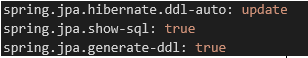
\includegraphics{AlgoritmoHibernate.png}}
\vspace{7mm}

Além disso, devem ser colocadas neste mesmo arquivo, os dados para se conectar no banco:

\vspace{7mm}
\centerline{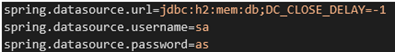
\includegraphics[width=80mm,height=600mm,keepaspectratio]{Postegresql.png}}
\vspace{7mm}

Com todos os pontos mencionados acima estando definidos, qualquer operação feita na API (criar, deletar, alterar, atualizar), será refletida automaticamente no banco de dados.
Além disso, é necessário adicionar as seguintes dependências no arquivo "pom.xml", para possibilitar a conexão com o banco PostgreSQL:

\vspace{7mm}
\centerline{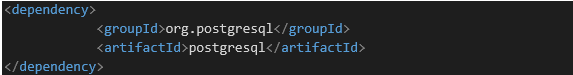
\includegraphics[width=80mm,height=200mm,keepaspectratio]{Postgresql2.png}}
\vspace{7mm}

Os endpoints (requisições http) da aplicação são definidos na pasta controller do projeto da API. Por padrão, o caminho da url é definido como “http://localhost:8080”, sendo que a porta 8080, é especificada na variável “server.port” que fica no arquivo de configuração “application-dev.properties”.

Para cada classe do Controller, foi adicionada a anotação “@RequestMapping” do spring boot que recebe como parâmetro a url principal da página.

Para subir a API para o heroku, inicialmente foi necessário criar um projeto através do endereço “heroku.com” e, após criado no menu “Deploy” foi selecionada a primeira opção denominada “Heroku Git”, sendo necessário instalar o programa Heroku CLI com a finalidade de conectar o git com o heroku.

\vspace{7mm}
\centerline{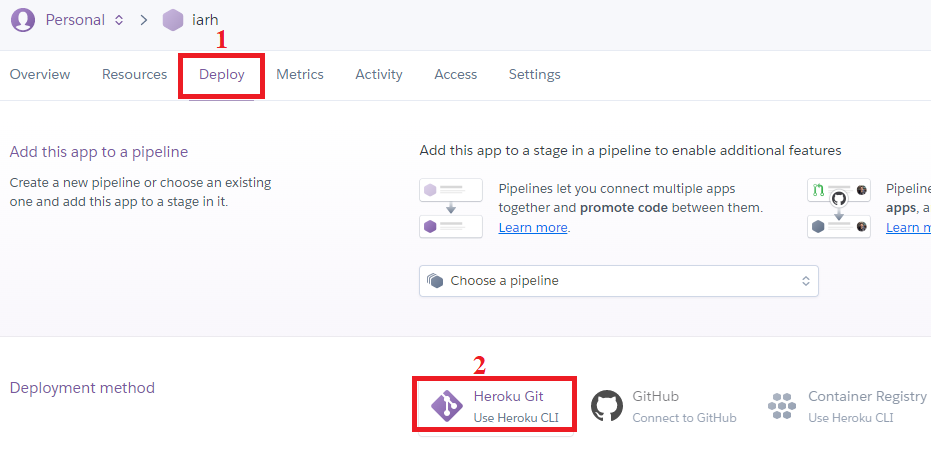
\includegraphics[width=80mm,height=600mm,keepaspectratio]{Heroku.png}}
\vspace{7mm}

Logo em seguida, foram executados os seguintes comandos no terminal, no diretório do projeto:

\begin{itemize}
\item heroku –version
\item heroku login
\item heroku git:remote -a nomedoprojeto
\item git status
\item git add .
\item git push heroku master
\end{itemize}

\section*{Resultados Obtidos}



\section*{Conclusão}
Com o trabalho proposto, foi possível aprender como desenvolver um aplicativo móvel, usando boas práticas de programação, além de compreender melhor o funcionamento da inteligência artificial aplicada no processo de seleção de candidatos, principalmente o método da regressão linear.

\begin{thebibliography}{00}
\bibitem{b1} F. Bo-Shone, "Technology, Jobs e the Future of Work in Australia", Julho 2021.
\bibitem{b2} M. Afonso Paulo, R. Brenno Anderson, A. Cristine Amora e V. Rosângela Couras, "INTELIGÊNCIA ARTIFICIAL - RECURSOS HUMANOS FRENTE AS NOVAS TECNOLOGIAS, POSTURAS E ATRIBUIÇÕES", Outubro 2018.
\bibitem{b4} T. Ivana, "The Attitude of Job Candidates towards Artificial Intelligence in Hiring Process", Maio 2020.
\bibitem{b5} S. Abhilasha e S. Apurva, "Impact of Artificial Intelligence on HR practices in the UAE".
\bibitem{b6} R. Geetha e D. Bhanu Sree, "RECRUITMENT THROUGH ARTIFICIAL INTELLIGENCE: A CONCEPTUAL STUDY ".
\bibitem{b7} J. Mariana Namen, "INTELIGÊNCIA ARTIFICIAL NO RECRUTAMENTO and SELEÇÃO:INOVAÇÃO E SEUS IMPACTOS PARA A GESTÃO DE RECURSOSHUMANOS", Fevereiro 2020.
\bibitem{b8} F. Krykhtime, A. Morim, N. Vale, L. Fortes e A. Neto, “Aplicando Lógica Fuzzy em um Modelo de Seleção Multicritério para Multiclientes”, Outubro 2013.
\bibitem{b9} E. Loiola, D. Silveira e M. Bittencourt, “E-Recruiting Utilizando Lógica Fuzzy”, Novembro 2022.
\bibitem{b10} L. Silva, “Modelos de Regressão Fuzzy”, 2018.
\end{thebibliography}
\vspace{12pt}

\end{document}
